\documentclass{sig-alternate-05-2015}
\usepackage{float}
\usepackage{enumitem}
\usepackage{subfiles}
\usepackage[english]{babel}
\usepackage{graphicx}
\usepackage{epstopdf}
\usepackage{tabularx}
\usepackage{url}
\usepackage{xcolor}
\usepackage{soul}
\setlist[description]{leftmargin=\parindent,labelindent=\parindent}
\makeatletter
\def\@copyrightspace{\relax}
\makeatother
\title{Design Concepts}
\begin{document}
\maketitle

\section{Interface Interaction}

There are several interface tasks that need to be performed. These are: Tool selection, Exporting/ Importing models, switching between views and type selection for use with the painting tool.
There are a small number of tools: Selection, line drawing, landmark placement and painting. Therefore, we can combine the tool selection and import/export functionality into a single wedge menu like the one in Figure 1.
\begin{figure}[H]
	\centering
	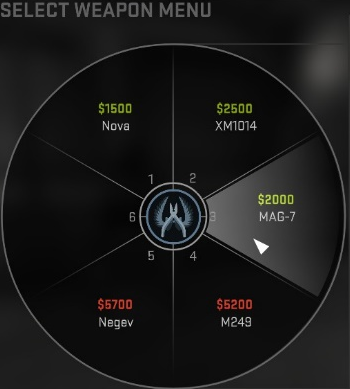
\includegraphics[width=5cm]{WedgeMenu}
	\caption{An example of a wedge menu used in the popular game CS: GO}
\end{figure}  This provides a 2DOF solution for selection from multiple objects. It is fast to use as a single button press is required to bring up the menu and one small movement in the correct direction is used to select an object\cite{Kurtenbach1993}. Additionally, by utilizing small movements we reduce user fatigue. It also allows for scaffolding such that experienced users can simply remember the direction of specific tools and choose not to visually display the menu\cite{Conner1992}. It does however, require a devoted button and in the case where there are many objects to choose from it may become unwieldy. However, it is a substantial improvement over a non-constrained menu or a menu that requires THI which could lead to fatigue. An alternative design for this sort of menu is to have the user rotate the menu to select the top object\cite{Hand1997}. While this is a 1DOF task we chose not to implement it as regular rotations may lead to repetitive strain injuries.
Because of the same reasons discussed above it seems sensible to use a separate wedge menu for the type selection when using the painting tool. It is possible to use the same button to bring this menu up as the main menu depending on whether the user has selected the painting tool. Alternatively, it is possible to use a separate button. If the same button is used it will be necessary to have an escape option in the painting type menu to switch to another default tool (selector). Using the same menu design helps maintain consistency within the interface. User preference for using a single button vs two buttons to access the different menus can be A/B tested during the user-based design phase.
Since there are only two views that the user can switch between and since this is likely to be a common task it makes sense to devote a single button to toggle views. This will be discussed in greater detail in the navigation section.

\section{Navigation}

As stated in the previous section there needs to be an effective way for the user to switch between First Person View(FPV) and God View(GV).  One consideration that must be made is that this is not a symmetrical action. Switching from GV to FPV requires the user to pick a target location for themselves to `land' at, however, switching from FPV to GV simply moves the user's viewpoint up and backwards from their current location. However, as we will discuss in the Environment Interaction section selecting a target is a core functionality that the application must provide while in GV. Therefore, the user can simply use this tool to select a target to shift to FPV at. Once the target is selected the user can press the toggle button to switch to a FPV at that location. Once in FPV a second press of the same button will take the user back to GV by essentially moving the viewpoint upwards and backwards from the current state. The final consideration to make in this area is how to animate these changes of viewpoint. The two main options are a zoom in/out animation or a fade in and out while the viewpoint switches. Zooming has the advantage of allowing the user to maintain a certain level of orientation and knowledge of surroundings. However, this may lead to simulator sickness. These two options will need to be A/B tested during the user-based design phase.

Navigation or viewpoint manipulation will need to be implemented differently in each view. In FPV we want to simulate the `player experience' as much as possible and therefore plan to implement travel based on a walking metaphor. This has the benefit of reducing the possibility of simulator sickness as well as simulating a player-like experience. Unfortunately, it is a somewhat slow method to travel over large distances and requires the terrain to be walkable. However, allowing the user to switch easily between views lets them switch to GV and select a new point to visit facilitating travel over large distances or past non-traversable terrain. Walking also has advantages over the other major options which are flying and direct teleportation. Flying can quite easily lead to simulator sickness and requires 3D movement which is often a significant cognitive burden for people and would require both joysticks. While we have some form of teleportation available via switching views, direct teleportation from within FPV has 2 drawbacks. Firstly, it requires the user to be in line of sight to select their destination (as well as controls devoted to target selection) and secondly it can lead to user disorientation upon a sudden viewpoint change. Walking requires a single joystick for movement and avoids these drawbacks. 
In GV we will use the world in hand metaphor as a technique of view point manipulation. The world will be directly mapped to the user's non-dominant hand(NDH). This will allow the user to rotate and move the world relative to a static view point. Using the world-in-hand metaphor allows the user to position the world such that other interactions can take place from a comfortable position. This reduces user fatigue and allows for natural gestures to be used for other forms of interaction. It is from GV that users will perform environment interaction. We will perform A/B testing to determine whether users prefer to turn off world manipulation during environment interaction or to continue to map the world's position and orientation to the NDH controller.
Another consideration we must make with the FPV is how users will be able to locate and orientate themselves in the VE. This is especially necessary if we are teleporting the user to a FPV without a zoom effect as they may be disorientated by the change in perspective. To facilitate this, we can use two navigational aides. Firstly, we can integrate access to a map in FPV as an option in the main menu, this will allow the user to identify their location and orientation. This will only be necessary if we find that user's are becoming too disorientated when entering FPV. Secondly while in GV the user will be able to place land marks using a special tool to indicate points of interest. These will be visible in FPV as large columns so that the user can easily locate these points. We chose not to implement a persistent mini-map in FPV as it would take up too much of the user's view. Another option for identifying points of interest in FPV is implementing a wayfinding arrow. However, this may take up too much space and is less useful for identifying the location of objects relative to a point of interest. Finally it can only point to a single point at once.

\section{Environment Interaction}
For environment interaction one of the principle functionalities of the application is the ability to select points and manipulate them across 3-Axis. There are two viable ways to select points, each corresponding to a different control technique. 
The first selection option is ray-casting. Here the user simply points using a controller (Dominant Hand (DH)) to select a point. Since this means the virtual representation of the user's hand is not necessarily close to the point it makes direct manipulation unnatural and difficult to implement consistently. We can therefore replicate a 3D widget representing the point in the virtual space near the user's hand and manipulate that directly, mirroring changes to the actual point on the terrain. The downside to this is the extra layer of abstraction as well as the difficulty of catering for how sensitive the widget should be with regards to controller movements. However, there has been research in this area where the speed at which the user moves the controller corresponds to the sensitivity, i.e. fast movements lead to large changes while slow movements lead to small changes.
The second selection technique is the go-go hand method where the user's hand is tracked non-linearly: the further it moves from the original position the larger the movements it makes in the virtual space. This allows the user to directly grasp points as a selection technique. Since the user's virtual hand is always on the point to be manipulated in this case it makes more sense to incorporate direct manipulation of the point on the terrain. However, there is once again the issue of sensitivity of the controls, especially with distant points. Additionally, this control scheme often results in the user working with their arms fully or mostly extended which can lead to fatigue issues.
Both techniques have several advantages and disadvantages, it will likely take a basic implementation of both to establish whether either or both are practically applicable. If both are viable then further testing will be done during the user-based design phase. Both techniques also would be implemented using similar physical controls. The DH controller would be used for selection (either for pointing or reaching). Once a point was selected the DH controller would be directly mapped to the widget control axes (movement in the vertical and horizontal axis and rotation around the depth axis). Exceptionally, points along a user drawn curve (discussed below) have variables that differ on opposite sides of the curve creating 5 independent variables. In this case, we will utilise THI to allow for consistent direct mapping. The DH will remain continue to determine the vertical axis variable. The NDH and DH hands will manipulate the horizontal axis and rotational variables on the side of the line they correspond to, i.e. the left hand will control the variables on the left of the line from the user's current view-point. It should be noted that in all cases movements that are not directly along a specific axis of movement or rotation will be ignored wrt editing environment variables.

It should be noted that while the techniques compete in this area ray-casting is more obviously superior for several other tasks mentioned below.
Other forms of environment interaction include painting on terrain types and drawing curves over the terrain on which points can be placed. These are, in fact, very similar and can both be implemented in a rather straightforward manner using ray-casting. This has the benefit over direct interaction of requiring far smaller movements thus reducing fatigue. The one drawback is that it may be hard to draw steady curves using ray-casting but this can be corrected using curve smoothing. With regards to the physical control requirements this can be implemented using the DH controller as a pointing device together with a button to indicate whether pen/brush is down. The implementation will be the same and the effect in the VE will be based on the tool selected.
\section{Tools and Descriptions}
\subsection{Main Menu}
\begin{description}
	\item[Select] This is the default tool. It will be selected when the user starts up the interface and when they return from using the paint tool. It allows the user to select points on the terrain. The user can select any point but if node is close to the point selected the node will be selected. If a node is selected this will bring up the interface elements for editing a node. To select a point the user points to it using ray-casting and pulls the DH bottom trigger. If a node is selected and the user wishes to deselect it they can press the bootom trigger button a second time. To delete a node the user may select it and then double click the bottom trigger. If a non-node point is selected a marker will be displayed to help the user track what location is selected.
	\item[Draw] Using this tool the user can either create nodes or sketch lines on the terrain surface. It works in a similar fashion to the select tool where the user uses ray-casting to point to a location on the terrain to draw a point or line there. To draw a point the user then taps the bottom DH trigger. If the user keeps the trigger held down they will then begin drawing a line. A line will automatically have a node at either end. If the user tries to create a node very close to an existing line the node will snap onto the line.
	\item[Paint] The paint tool allows the user to paint a variety of terrain types onto the terrain. When the paint tool is selected users will be able to access an extra type menu which allows them to select which terrain type they paint (more detail in section 4.2). To use the paint tool users again select a location on the terrain using ray-casting. The paintbrush can either be up or down depending on whether the bottom trigger on the DH controller is depressed or not respectively. To set the width of the brush tool users can use the "A" button on the DH controller to widen it and the "B" button to narrow it.
	\item [Landmark] The landmark tool allows the user to place landmarks on the terrain for use in FPV. It will function in the same manner as the draw tool except landmarks will be placed instead of nodes.
	\item[Import] This tool allows the user to import existing terrain designs. Save files will be accessed via the standard OS interface as it is outside the scope of this project to create custom interfaces for this.
	\item[Export] This tool allows the user to export the current terrain design. Save files will be created via the standard OS interface as it is outside the scope of this project to create custom interfaces for this.
\end{description}
\subsection{Paint Menu}
When the paint tool is selected this menu will be available to the user to select a terrain type or to exit the paint tool.

\begin{description}
	\item[Type /[x/]] Selects the terrain type the user will paint onto the terrain using the paint tool
	\item [Back] Exits the paint tool and switches to the select tool.
\end{description}
\section{Paper Prototype}
\subsection{Design}
The paper prototype allowed the user to interact with all UI elements that were planned to be included in the VE interface. It also included a number of user instructions to guide first time uses through the program. Although the interface elements would react to user input it was not feasible to have the terrain model itself to react. Thus users were required to imagine how the terrain would change based on verbal feedback.

The prototype was constructed using a number of parts to represent various interface elements. The displayed terrain itself was represented by a flat sheet of paper on a table surface. This allowed UI elements to be placed onto the terrain surface in approximation to the functionality of the VE. Users were asked to keep in mind that the terrain image was simply a representation of the VR display. A number of UI elements were represented by small cardboard tokens which could be placed on the terrain or "view area". Two ring menus were included, one being the main menu which users could select tools with and the other being \hl{a terrain type menu which users could use to select a type of terrain to paint onto the terrain}. There were also landmark and teleport target markers that the user could place onto the terrain. 
A small cardboard hand was used to help users keep track of their hand within the VE during menu interaction. However, this was not present during other interactions. This was identified as a weakness in the prototype after evaluations had taken place. Within the VE the user would have constantly visible hand avatars which help them track their hand positions and orientations. Since this was lacking in the prototype users would often reset their hands to a rest position without considering the effect this would have on their current interaction.
When interacting with the terrain users were asked to point with their index finger to represent the functionality of ray-casting, this closely approximate how the ray-casting feature of the interface will work. When using the paint tool users were shown outlines of the area they would paint on the terrain by a hollow paper ring placed on top of the terrain.

Point and line constraints on the terrain were simulated using blue putty. This added a 3 dimensional aspect to the prototype while allowing users to create an arbitrary number of point constraints and any length or shape of line constraints. Additionally, the interactive point widget was represented by a ball of putty with 3 wooden arms which could be manipulated by the user to edit the properties of the constraint. This closely approximated the widgets in the desktop application pictured below.

\begin{figure}[H]
	\centering
	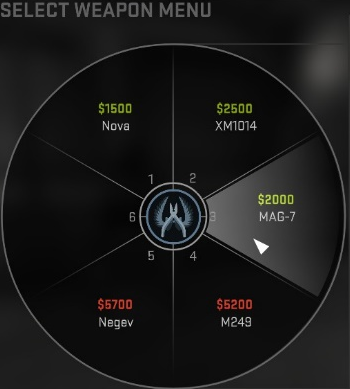
\includegraphics[width=5cm]{WedgeMenu}
	\caption{An example of a wedge menu used in the popular game CS: GO}
\end{figure}

\subsection{Evaluation}
\subsection{Changes to design}
\bibliographystyle{abbrv}
\bibliography{proposal}
\end{document}